\subsection{Data Layering}

We have a system which is able to support end-to-end encryption of data with permissions and access control. As an extension of this, we briefly consider how this data might be layered such that different parties see different views of data.

As an example, take the following JSON object in program code \ref{code:patient_record_json}. Let's assume this represents a record of a patient visiting a general practitioner.

\begin{listing}[H]
  \centering
  \begin{minted}{json}
{
  "doctor": {
    "id": 01234567,
    "name": "Dr. So So"
  },
  "metadata": {
    "created": "2017-01-01T10:05:00+00:00",
    "modified": "2017-01-01T10:11:12+00:00"
  },
  "notes": "..."
}
  \end{minted}
  \caption{
  	An example patient record
  }
  \label{code:patient_record_json}
\end{listing}


Now let's split the JSON object into three further JSON objects corresponding to the "doctor", "metadata", and "notes" properties. We could also do the same to the "doctor" and "metadata" objects. This would result in five separate JSON objects which, when combined, form the original JSON object. This is a recursively applied process.

\subsubsection{Storing data chunks}

Since the structure of a JSON object is representative of a tree, when evaluated as above, we can use this property to visualise the data as a file system:

\begin{figure}[H]
  \centering
  \includegraphics[width = 6cm]{images/json_file_structure.png} \\
  \caption{
  	JSON represented by file structure
  }{
    The use of the suffix '.part' denotes a file representing a property of the parent JSON object.
  }
  \label{fig:json_file_structure}
\end{figure}

The use of the suffix '.part' hints at an file representing a property of the parent JSON object. We can transform the tree in figure \ref{fig:json_file_structure} into a Merkle tree by taking the hash of each file. Given the file content in program code \ref{code:patient_record_json} the resulting Merkle tree is shown in figure \ref{tikz:json_merkle_tree}.

\begin{figure}[H]
  \centering
  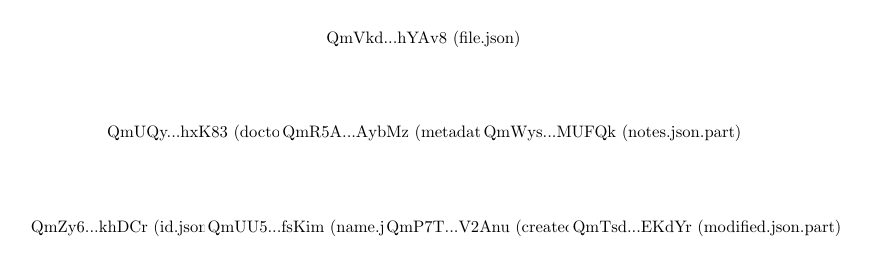
\begin{tikzpicture}[scale = 0.6, every node/.style={scale = 0.6}, every node/.append style={fill = white, rounded corners = 2pt, inner sep = 2pt, align = center}]

  \node at (0, 0) { QmVkd...hYAv8 (file.json) };

  \node at (-4, -2) { QmUQy...hxK83 (doctor.json.part) };
  \node at (0, -2) { QmR5A...AybMz (metadata.json.part) };
  \node at (4, -2) { QmWys...MUFQk (notes.json.part) };

  \node at (-6, -4) { QmZy6...khDCr (id.json.part) };
  \node at (-2, -4) { QmUU5...fsKim (name.json.part) };

  \node at (2, -4) { QmP7T...V2Anu (created.json.part) };
  \node at (6, -4) { QmTsd...EKdYr (modified.json.part) };

  \end{tikzpicture}
  \caption{
    Merkle tree of a JSON file
  }
  \label{fig:json_merkle_tree}
\end{figure}


\subsubsection{Permissions for data chunks}
